\section{Bayesian Dirichlet quotient score}

\cite{Suzuki2017} independently suggested a Bayesian Dirichlet
quotient score BDq, in which the NML-distributions
$P^1_{NML}(D_{i,G_i};G)$ and $P^1_{NML}(D_{G_i};G)$ of the qNML are
replaced by the Bayesian marginal likelihoods
$P^1(D_{i,G_i};G,\alpha)$ and $P^1_{NML}(D_{G_i};G,\alpha)$ using
parameter prior $\theta_{ij} \sim
Dirichlet(\alpha,\ldots,\alpha)$. Suzuki further suggested using the
Jeffreys' prior with $\alpha=\frac{1}{2}$. While this is a
popular choice in statistics, it is also possible to argue for other
values of $\alpha$ like $\alpha=\frac{1}{2}-\frac{\ln 2}{2\ln
  N}$~\citep{watanabe15a} and $\alpha=\frac{1}{3}$~\citep{jaasaari18}.

Our initial experiments indicate that model selection by BDq is still
highly sensitive to the hyperparameter $\alpha$. On the next 5 pages we
present results for learning the posterior distribution of the network
structures for the four predictor variables (discretized to three
equal width bins) in the iris data (N=150). The structure prior is
assumed to be uniform. Since BDq is score equivalent, we only include
one representative from each equivalence class. The images also show
the most probable structure and the predictive distribution given by
the most probable structure and the predictive distribution when
marginalizing over all the structures.


One can see how the structure posterior is quite sensitive to $\alpha$
and the selected network is different for $\alpha$-values $0.2$, $0.3$
and $0.5$.

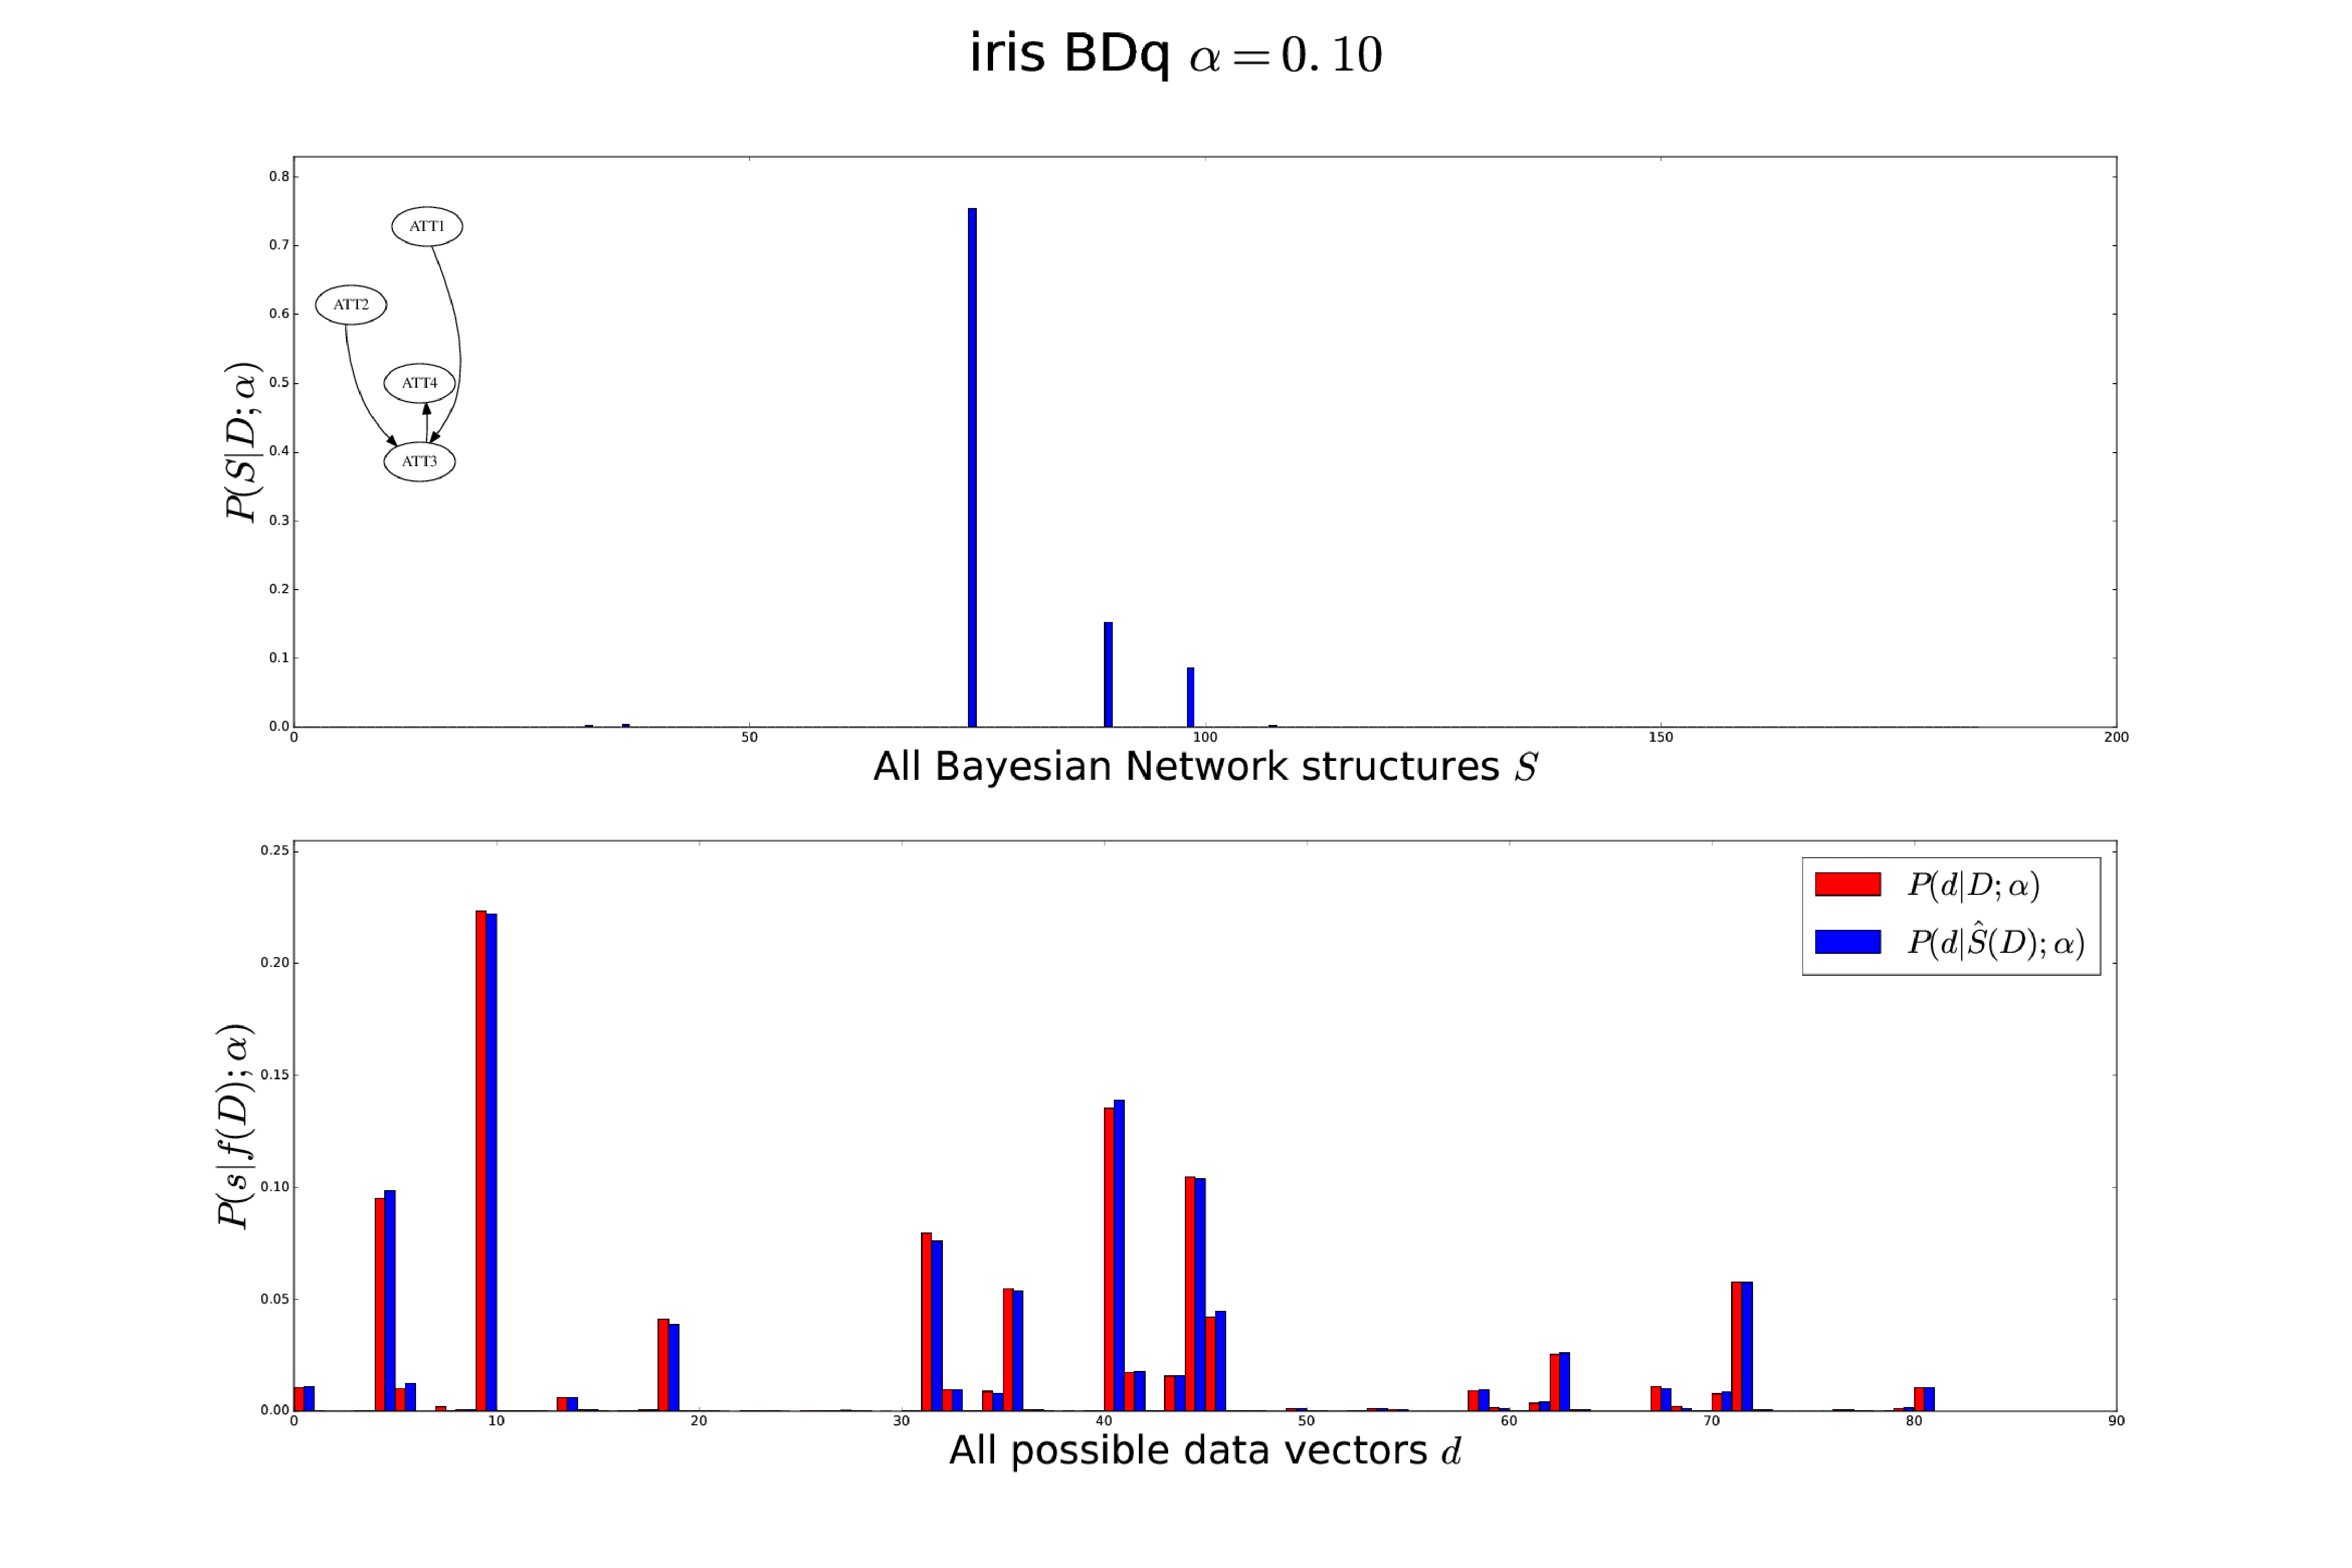
\includepdf[pages={1-5},angle=90]{qsens.pdf}


